We relate the duality framework to finite-dimensional IQC multipliers and
apply the resulting synthesis conditions to a delayed neural population
model.

\subsection{Positive--negative multipliers}

Let $\R H_\infty$ denote the proper real-rational transfer matrices with
no poles in the closed right half-plane. For
$\Psi\in\R H_\infty^{(n_{\tilde z}+n_{\tilde w})\times(n_z+n_w)}$,
define the para-Hermitian adjoint by
\begin{equation*}
 \Psi^\sim(i\omega)=\Psi(-i\omega)^\top
 \in\mathbb C^{(n_z+n_w)\times(n_{\tilde z}+n_{\tilde w})}.
\end{equation*}
Given a constant symmetric matrix
$V\in\R^{(n_{\tilde z}+n_{\tilde w})\times(n_{\tilde z}+n_{\tilde w})}$,
partition $\Pi=\Psi^\sim V\Psi$ according to the input dimensions
$n_z$ and $n_w$, so that \(
 \Pi(i\omega)\in\mathbb C^{(n_z+n_w)\times(n_z+n_w)},\\
\)
We say that $\Pi$ is strict positive--negative (PN)
if there exists $\epsilon>0$ such that
\begin{equation*}
 \begin{gathered}
 \Pi(i\omega)=
 \bmat{\Pi_{11}(i\omega)&\Pi_{12}(i\omega)\\
       \Pi_{12}(i\omega)^*&\Pi_{22}(i\omega)},\\
 \Pi_{11}(i\omega)\succeq\epsilon I_{n_z},\qquad
 \Pi_{22}(i\omega)\preceq-\epsilon I_{n_w}
 \end{gathered}
\end{equation*}
for all $\omega\in\R\cup\{\infty\}$. By~\cite[Thm.~4]{6915700}, a
strict PN multiplier admits a square $J$-spectral factor
\begin{equation*}
\Pi=\Theta^\sim J\Theta,
 \qquad J=\operatorname{diag}(I_{n_z},-I_{n_w}),
\end{equation*}
with $J\in\R^{(n_z+n_w)\times(n_z+n_w)}$ and
$\Theta,\Theta^{-1}\in\R H_\infty^{(n_z+n_w)\times(n_z+n_w)}$.
Moreover, this $J$-spectral factorization satisfies
$\Theta_{22}^{-1}\in\R H_\infty^{n_w\times n_w}$. Thus the invertibility requirements in
Definition~\ref{def:factorization} hold, and the dual filter is
$\mbf D(\Theta)\in\R H_\infty^{(n_w+n_z)\times(n_w+n_z)}$. The Riccati construction 
in~\cite[App.~B]{Pfifer2015} uses the factorization results of~\cite{MEINSMA1995243}
and provides a computational method to find factorizations. Related
finite-horizon formulations ~\cite{carrasco2018equivalence,scherer2018dynamicdissipation}.

\subsection{Robust stabilization of the STN--GPe network}
We consider the delayed firing-rate model
of~\cite[Eq.~(5)]{nevadoHolgado2010betaOscillations} with $K_d =1$, i.e. the diseased case.
Let $\mrm{STN}$ and
$\mrm{GP}$ denote the firing rates of the subthalamic nucleus (STN) and
globus pallidus pars externa (GPe), respectively, and replace $I_{\mrm{e}}\mrm{Stim}$
with $ u(t)$. The plant is
\begin{equation}
      \begin{aligned}
      \tau_{\mrm{S}} \dot{\mrm{STN}}(t)
          ={}&F_{\mrm{S}}\!\bigl(-w_{\mrm{GS}}\mrm{GP}
              (t-\tau_{\mrm{GS}})\\
             &\qquad\quad +w_{\mrm{CS}}\mrm{Ctx}\bigr)
              -\mrm{STN}(t)+ u(t),\\
      \tau_{\mrm{G}} \dot{\mrm{GP}}(t)
          ={}&F_{\mrm{G}}\!\bigl(w_{\mrm{SG}}\mrm{STN}
              (t-\tau_{\mrm{SG}})\\
             &\qquad\quad-w_{\mrm{GG}}\mrm{GP}(t-\tau_{\mrm{GG}})\\
             &\qquad\quad-w_{\mrm{XG}}\mrm{Str}\bigr)-\mrm{GP}(t).
      \end{aligned}
\end{equation}
The activation functions $F_i\colon\R\to\R$ are
\begin{equation}\label{eq:stn-gpe-uncentered-sigmoid}
F_i(q)=\frac{M_i}{1+\exp(-4q/M_i)(M_i-B_i)/B_i},
\qquad i\in\{\mrm{S},\mrm{G}\},
\end{equation}
with $F_i(0)=B_i$. Define the sigmoid midpoint and centered activation
$\sigma_i\colon\R\to\R$ by
\begin{equation}\label{eq:stn-gpe-centered-sigmoid}
\begin{aligned}
c_i&:=\frac{M_i}{4}\ln\!\left(\frac{M_i-B_i}{B_i}\right),\\
\sigma_i(q)&:=\frac{M_i}{1+\exp(-4q/M_i)}-\frac{M_i}{2}=\frac{M_i}{2}\tanh\!\left(\frac{2q}{M_i}\right).
\end{aligned}
\end{equation}
Then $F_i(q)=\sigma_i(q-c_i)+M_i/2$. With the centered states
\begin{equation*}
\tilde{x}_{\mrm{S}}:=\mrm{STN}-\frac{M_{\mrm{S}}}{2},
\qquad
\tilde{x}_{\mrm{G}}:=\mrm{GP}-\frac{M_{\mrm{G}}}{2},
\end{equation*}
and offsets
\begin{equation*}
\begin{aligned}
b_{\mrm{S}}&:=w_{\mrm{CS}}\mrm{Ctx}-\frac{w_{\mrm{GS}}M_{\mrm{G}}}{2}-c_{\mrm{S}},\\
b_{\mrm{G}}&:=\frac{w_{\mrm{SG}}M_{\mrm{S}}}{2}-\frac{w_{\mrm{GG}}M_{\mrm{G}}}{2}
      -w_{\mrm{XG}}\mrm{Str}-c_{\mrm{G}},
\end{aligned}
\end{equation*}
the plant becomes
\begin{equation}\label{eq:stn-gpe-centered}
\begin{aligned}
\tilde{z}_{\mrm{S}}(t)&:=-w_{\mrm{GS}}\tilde{x}_{\mrm{G}}(t-\tau_{\mrm{GS}})+b_{\mrm{S}},\\
\tilde{z}_{\mrm{G}}(t)&:=w_{\mrm{SG}}\tilde{x}_{\mrm{S}}(t-\tau_{\mrm{SG}})
          -w_{\mrm{GG}}\tilde{x}_{\mrm{G}}(t-\tau_{\mrm{GG}})+b_{\mrm{G}},\\
\tau_{\mrm{S}}\dot{\tilde{x}}_{\mrm{S}}(t)
      &=\sigma_{\mrm{S}}(\tilde{z}_{\mrm{S}}(t))
        -\tilde{x}_{\mrm{S}}(t)+\tilde{u}(t),\\
\tau_{\mrm{G}}\dot{\tilde{x}}_{\mrm{G}}(t)
      &=\sigma_{\mrm{G}}(\tilde{z}_{\mrm{G}}(t))
        -\tilde{x}_{\mrm{G}}(t).
\end{aligned}
\end{equation}
where $\sigma_i(0)=0$. Here $\tau_{ij}$ and $w_{ij}$ denote the transmission
delay and synaptic weight from population $i$ to population $j$, while
$\tau_{\mrm{S}}$ and $\tau_{\mrm{G}}$ are the population time constants.
Let $(\tilde x_{\mrm{S}}^\star,\tilde x_{\mrm{G}}^\star)$ be an equilibrium
satisfying
\begin{align*}
      \tilde z_{\mrm{S}}^\star&:=-w_{\mrm{GS}}\tilde x_{\mrm{G}}^\star+b_{\mrm{S}},\\
      \tilde z_{\mrm{G}}^\star&:=w_{\mrm{SG}}\tilde x_{\mrm{S}}^\star
          -w_{\mrm{GG}}\tilde x_{\mrm{G}}^\star+b_{\mrm{G}},\\
      \tilde x_{\mrm{S}}^\star
          &=\sigma_{\mrm{S}}(\tilde z_{\mrm{S}}^\star),\\
      \tilde x_{\mrm{G}}^\star
          &=\sigma_{\mrm{G}}(\tilde z_{\mrm{G}}^\star).
\end{align*}
For $i\in\{\mrm{S},\mrm{G}\}$, introduce the deviation variables
\begin{equation*}
x_i(t):=\tilde{x}_i(t)-\tilde x_i^\star,
\quad
z_i(t):=\tilde{z}_i(t)-\tilde z_i^\star,
\end{equation*}
and define the shifted nonlinearities $\delta_i\colon\R\to\R$ by
\begin{equation*}
\delta_i(v):=\sigma_i(\tilde z_i^\star+v)-\sigma_i(\tilde z_i^\star).
\end{equation*}
Following~\cite{peet2020representationnetworkssystemsdelay}, introduce
the delayed states $\phi_{ij}(t,s):=x_i(t-\tau_{ij}s)$ for
$(i,j)\in\mcl I_{\mrm{D}}$ and $s\in[0,1]$, where
$\mcl I_{\mrm{D}}:=\{(\mrm{G},\mrm{S}),(\mrm{S},\mrm{G}),(\mrm{G},\mrm{G})\}$.
The shifted plant has the equivalent ODE--PDE representation
\begin{equation}\label{eq:stn-gpe_ode-pde}
\begin{aligned}
z_{\mrm{S}}(t)
    &:= -w_{\mrm{GS}}\phi_{\mrm{GS}}(t,1),\\
z_{\mrm{G}}(t)
    &:= w_{\mrm{SG}}\phi_{\mrm{SG}}(t,1)
        -w_{\mrm{GG}}\phi_{\mrm{GG}}(t,1),\\
\tau_{\mrm{S}}\dot{x}_{\mrm{S}}(t)
    &= \delta_{\mrm{S}}(z_{\mrm{S}}(t))-x_{\mrm{S}}(t)+u(t),\\
\tau_{\mrm{G}}\dot{x}_{\mrm{G}}(t)
    &= \delta_{\mrm{G}}(z_{\mrm{G}}(t))-x_{\mrm{G}}(t),\\
\dot{\phi}_{ij}(t,s)
    &= -\frac{1}{\tau_{ij}}\phi_{ij,s}(t,s),\\
\phi_{ij}(t,0)
    &= x_i(t),\qquad (i,j)\in\mcl I_{\mrm{D}}.
\end{aligned}
\end{equation}
The equilibrium is now at the origin, and the shift affects only the
nonlinearities $\delta_i$. We synthesize feedback through $u$ to robustly
stabilize this equilibrium.

\subsection{Robust stability}

The diagonal uncertainty acting on two-dimensional signals is
$\Delta=\operatorname{diag}(\delta_{\mrm S},\delta_{\mrm G})$. It is memoryless,
monotone, and zero at the origin. We compare a static sector IQC with a
Zames--Falb IQC~\cite{zames1968stability,
turner2022zamesfalbmultipliersdontpanic}. For each channel, let
$M,H\in\R H_\infty$ satisfy $M=1-H$
with
\begin{equation*}
 H(\omega)=\sum_{k=1}^3\frac{\kappa_{k}}{i\omega+a_{k}},
 \qquad a_{k}>0,\quad\kappa_{k}\geq0.
\end{equation*}
The nonnegative impulse response $h_i$ satisfies
$\|h\|_{L_1}=\sum_k\kappa_{k}/a_{k}<1$, so the multiplier is valid for
monotone slope-restricted nonlinearities without requiring oddness. We
choose the same coefficients for both channels, using the population time
constants $\tau_{\mrm S}= \tau_\mrm{GS} = \tau_\mrm{SG}=6\,\mathrm{ms}$ and
$\tau_{\mrm G}=14\,\mathrm{ms}$ and the recurrent GPe delay
$\tau_{\mrm{GG}}=4\,\mathrm{ms}$. Specifically,
\begin{equation*}
 (a_{1},a_{2},a_{3})
 =\left(\frac{1}{\tau_{\mrm G}},\frac{1}{\tau_{\mrm S}},
          \frac{1}{\tau_{\mrm{GG}}}\right)
\end{equation*}
Thus the multiplier poles are $-a_{k}$. We weigh the three modes by the corresponding synaptic
strengths related to $K_d=1$ are $w_\mrm{GS} = 10.7$, $w_\mrm{SG}=20.0$, and $w_\mrm{GG}=12.3$,
\begin{equation*}
 \begin{aligned}
 (r_1,r_2,r_3)&:=
 \frac{(w_{\mrm{GS}},w_{\mrm{SG}},w_{\mrm{GG}})}
 {w_{\mrm{GS}}+w_{\mrm{SG}}+w_{\mrm{GG}}}\\
 \kappa_{k}&:=\frac{10}{15}r_k a_{k}.
 \end{aligned}
\end{equation*}
This gives $\|h\|_{L_1}=\sum_k\kappa_{k}/a_{k}=10/15<1$.
The time scales and synaptic weights specify a fixed heuristic multiplier
shape, its coefficients are held fixed during the search over $\alpha$.
For each candidate bound $0<\alpha\leq1$, the multiplier
$\Pi_\mrm{ZF}(i\omega)\in\mathbb C^{2\times2}$ before regularization is
\begin{equation*}
 \Pi_\mrm{ZF}(i\omega)=
 \bmat{0&\alpha M(i\omega)^\sim\\
       \alpha M(i\omega)&-(M(i\omega)+M(i\omega)^\sim)}.
\end{equation*}
Since the upper-left
entry is zero, $\Pi_\mrm{ZF}$ is not strict PN. Both uncertainty classes
satisfy $|\delta_i(v)|\leq|v|$ and hence the IQC can be regularized with
weight $\bmat{\epsilon & 0 \\ 0 & -\epsilon}$ for some $\epsilon >0$
\begin{equation*}
 \Pi_{\epsilon}=\Pi_\mrm{ZF}
       + \bmat{\epsilon & 0 \\ 0 & -\epsilon},
\end{equation*}
the resulting multiplier remains a valid IQC and satisfies the strict PN requirement. 
Thus the multiplier and admits the hard $J$-spectral factor used in the dual-filter
construction. The static sector case follows with from Lemma~\ref{lem:sec-bound}.

\subsubsection{Admissible trajectories}
Performing bisection searches where we apply the same sector and slope restrictions
on $\delta_\mrm{S},\delta_\mrm{G}$ yield the certified bounds
\begin{equation*}
 \alpha_{\mrm{sec}}^\star=0.492,\qquad
 \alpha_{\mrm{ZF}}^\star=0.562.
\end{equation*}
For $i\in\{\mrm S,\mrm G\}$, the sector condition on an interval
$ I_i$ containing zero is
\begin{equation*}
 0\leq\frac{\delta_i(v)}{v}\leq\alpha_{\mrm{sec}}^\star,
 \qquad v\in I_{\mrm{sec},i}\setminus\{0\}.
\end{equation*}
The Zames--Falb multiplier uses the slope condition
\begin{equation*}
 0\leq\frac{\delta_i(v)-\delta_i(w)}{v-w}\leq\alpha_{\mrm{ZF}}^\star,
 \qquad v,w\in I_{\mrm{slope},i},\quad v\neq w.
\end{equation*}
Since the shifted sigmoids are smooth, the latter is equivalent to
$0\leq\delta_i'(v)\leq\alpha_{\mrm{ZF}}^\star$ on $ I_i$.
For each constraint, the maximal interval containing zero determines the
admissible trajectories $z_\mrm{S},z_\mrm{G}$ corresponding to the $K_d=1$ equilibrium is shown in
Figure~\ref{fig:stn-gpe-admissible-trajectories}.

\begin{figure}[H]
 \centering
 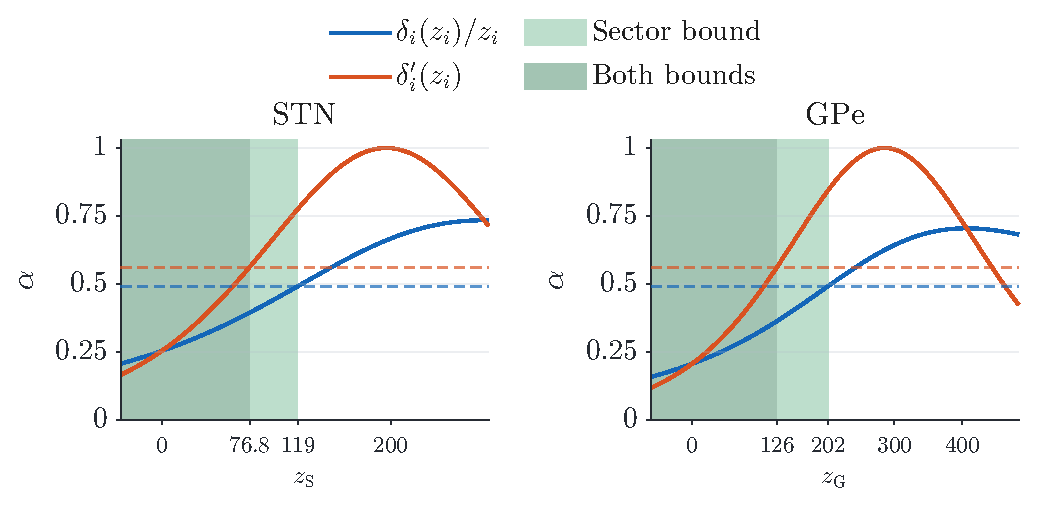
\includegraphics[width=\columnwidth]{Figures/stn_gpe_admissible_trajectories.pdf}
 \caption{Sector bounds (blue) and slope bounds (orange) for the shifted STN and GPe nonlinearities. 
 The dashed horizontal lines indicate the maximum certified values $\alpha_{\mrm{sec}}^\star=0.492$ 
 and $\alpha_{\mrm{ZF}}^\star=0.562$ obtained using the sector and Zames--Falb multipliers, 
 respectively. The shaded regions indicate the ranges of $z_{\mrm G}$ and $z_{\mrm S}$ for which 
 robust stability can be guaranteed. Although the Zames--Falb multiplier certifies a larger value of 
 $\alpha$, i.e., $\alpha_{\mrm{sec}}^\star < \alpha_{\mrm{ZF}}^\star$, the corresponding admissible 
 trajectory interval is smaller. This can be seen from the sector-bounded regions in the figure, 
 including the region in which both bounds are satisfied.
 }
 \label{fig:stn-gpe-admissible-trajectories}
\end{figure}


\subsubsection{Closed-loop simulation}

Figure~\ref{fig:stn-gpe-sector-trajectories} shows the shifted nonlinear response
with the controller synthesized using only the static sector IQC and the
robust-stability condition, at the certified value
$\alpha_{\mrm{sec}}^\star=0.492$. The initial condition is
$x_{\mrm S}(0)=x_{\mrm G}(0)=0$, with zero delay states, corresponding to
the original equilibrium.
To perturb the
$K\star P\star\Delta$ interconnection, we add a pulse in interconnection~\eqref{eqn:rob-stab-interconnect},
$w_\Delta(t)=\Delta(z_\Delta)+d$, where
\begin{equation*}
 d(t)=\begin{cases}
 \bmat{10\\-10}\sin^2\!\left(\dfrac{\pi(t-0.10)}{0.04}\right),
      &0.10\leq t\leq0.14,\\
 0, &\text{otherwise}.
 \end{cases}
\end{equation*}
The horizontal lines mark the sector
limits $z_i^{\max}$, defined by the first positive crossing of
$\delta_i(z_i)/z_i=0.4921875$.
The simulated closed-loop inputs remain below these limits, and the state
deviations return to zero after the disturbance.
Since $u=I_{\mrm e}\mrm{Stim}$ is added to the
firing-rate dynamics, it is an effective rate input, measured in spikes per
second rather than electrical current. The peak control effort is
$\max_t|u(t)|=19.15\,\mathrm{spikes/s}$. Converting this value to amperes
requires a separate calibration of $I_{\mrm e}$.

\begin{figure}[t]
 \centering
 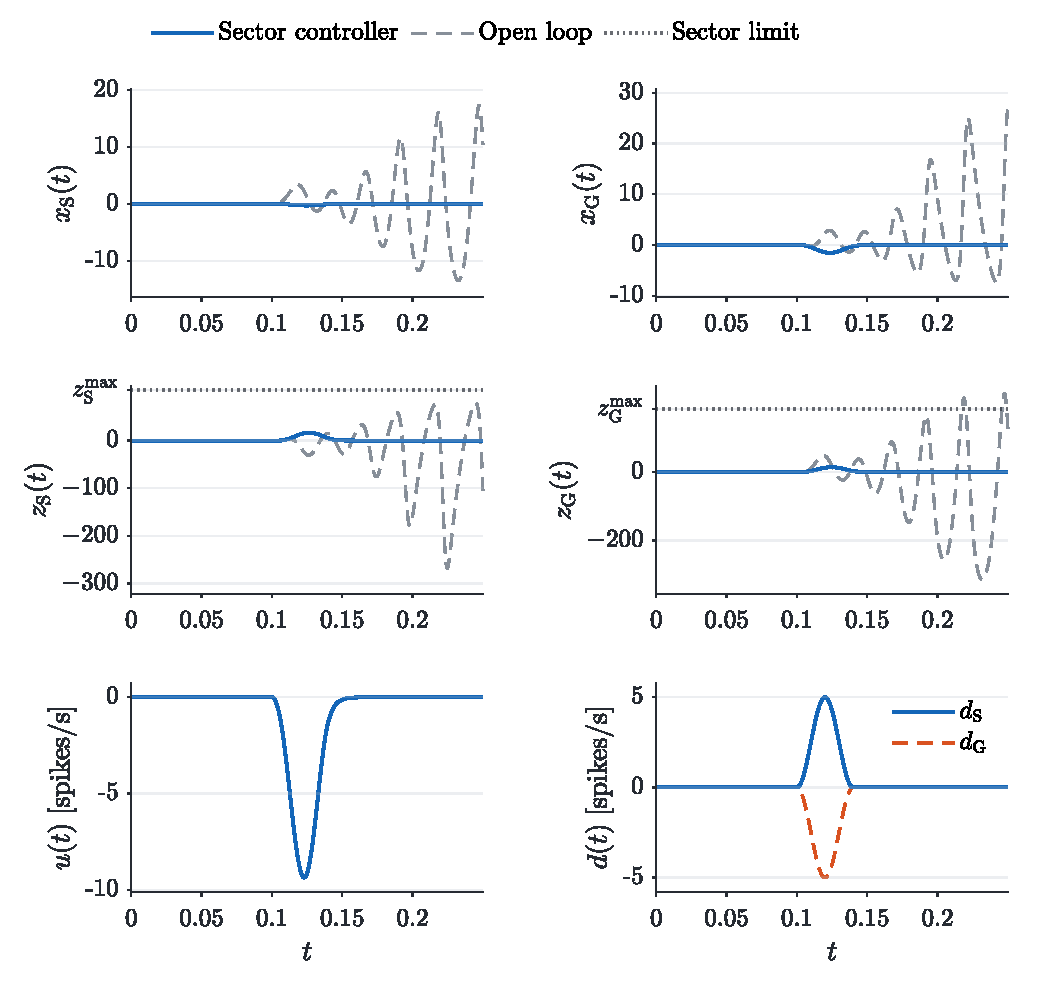
\includegraphics[width=\columnwidth]{Figures/stn_gpe_sector_trajectories.pdf}
 \caption{Shifted nonlinear STN--GPe simulation with the controller synthesized using the sector IQC.
  The top panels show the firing-rate deviations of the STN and GPe populations. The middle panels show the
  shifted nonlinearity inputs, $z_{\mrm S}(t)$ and $z_{\mrm G}(t)$, together with their sector-admissible
  upper limits, $z_{\mrm S}^{\max}=119.09$ and $z_{\mrm G}^{\max}=201.85$. Both inputs remain within
  the certified robust-stability region throughout the simulation. The bottom panels show the control 
  effort and the injected disturbance, respectively. The disturbance (bottom right) consists of 
  $d_{\mrm S}(t)$ (blue) and $d_{\mrm G}(t)$ (dashed orange).
}
 \label{fig:stn-gpe-sector-trajectories}
\end{figure}
